\documentclass[letterpaper]{article}
\usepackage[margin=1in]{geometry}
\usepackage[utf8]{inputenc}
\usepackage{textcomp}
\usepackage{amssymb}
\usepackage{natbib}
\usepackage{graphicx}
\usepackage{gensymb}
\usepackage{amsthm, amsmath, mathtools}
\usepackage[dvipsnames]{xcolor}
\usepackage{enumerate}
\usepackage{mdframed}
\usepackage[most]{tcolorbox}
\usepackage{csquotes}
% https://tex.stackexchange.com/questions/13506/how-to-continue-the-framed-text-box-on-multiple-pages

\tcbuselibrary{theorems}

\newcommand{\R}{\mathbb{R}}
\newcommand{\Z}{\mathbb{Z}}
\newcommand{\N}{\mathbb{N}}
\newcommand{\Q}{\mathbb{Q}}
\newcommand{\C}{\mathbb{C}}
\newcommand{\code}[1]{\texttt{#1}}
\newcommand{\mdiamond}{$\diamondsuit$}
\newcommand{\PowerSet}{\mathcal{P}}
\newcommand{\Mod}[1]{\ (\mathrm{mod}\ #1)}
\DeclareMathOperator{\lcm}{lcm}

%\newtheorem*{theorem}{Theorem}
%\newtheorem*{definition}{Definition}
%\newtheorem*{corollary}{Corollary}
%\newtheorem*{lemma}{Lemma}
\newtheorem*{proposition}{Proposition}


\newtcbtheorem[number within=section]{theorem}{Theorem}
{colback=green!5,colframe=green!35!black,fonttitle=\bfseries}{th}

\newtcbtheorem[number within=section]{definition}{Definition}
{colback=blue!5,colframe=blue!35!black,fonttitle=\bfseries}{def}

\newtcbtheorem[number within=section]{corollary}{Corollary}
{colback=yellow!5,colframe=yellow!35!black,fonttitle=\bfseries}{cor}

\newtcbtheorem[number within=section]{lemma}{Lemma}
{colback=red!5,colframe=red!35!black,fonttitle=\bfseries}{lem}

\newtcbtheorem[number within=section]{example}{Example}
{colback=white!5,colframe=white!35!black,fonttitle=\bfseries}{def}

\newtcbtheorem[number within=section]{note}{Important Note}{
        enhanced,
        sharp corners,
        attach boxed title to top left={
            xshift=-1mm,
            yshift=-5mm,
            yshifttext=-1mm
        },
        top=1.5em,
        colback=white,
        colframe=black,
        fonttitle=\bfseries,
        boxed title style={
            sharp corners,
            size=small,
            colback=red!75!black,
            colframe=red!75!black,
        } 
    }{impnote}
\usepackage[utf8]{inputenc}
\usepackage[english]{babel}
\usepackage{fancyhdr}
\usepackage[hidelinks]{hyperref}

\pagestyle{fancy}
\fancyhf{}
\rhead{CSE 101}
\chead{Monday, January 10, 2022}
\lhead{Lecture 4}
\rfoot{\thepage}

\setlength{\parindent}{0pt}

\begin{document}

\section{Directed Graphs}
A directed graph can be thought of as a graph of dependencies. For example, consider the following activities:
\begin{verbatim}
    Breakfast                       Go to work

                Wake up 

    Shower                          Dress 
\end{verbatim}
Of course, you can't do all five of these activities at the same time; there are some dependencies. Some of them are: 
\begin{itemize}
    \item Wake Up \textrightarrow{} Breakfast \textrightarrow{} Go to Work. 
    \item Wake Up \textrightarrow{} Go to Work. 
    \item Wake Up \textrightarrow{} Shower \textrightarrow{} Dress \textrightarrow{} Go to Work. 
\end{itemize}
In other words, you need to do $A$ before you can do $B$, and so on. One of the things we might want to do is order this graph in a way that respects these dependencies.

\subsection{Topological Ordering}
Essentially, a directed graph can be thought of as a graph of dependencies. An edge $v \mapsto w$ means that $v$ should come before $w$. We can use something known as topological ordering to better understand this relationship.

\begin{definition}{Topological Ordering}{}
    A \textbf{topological ordering} of a directed graph is an ordering of the vertices so that for each edge $(v, w)$, $v$ comes before $w$ in the ordering.
\end{definition}
A question that we might have is: does every directed graph have a topological ordering?
\begin{itemize}
    \item No. Consider the classic counterexample:
    \[\text{Chicken } \mapsto \text{ Egg}\]
    \[\text{Egg } \mapsto \text{ Chicken}\]
    In other words, there is a \emph{cycle} where the chicken goes to the egg and the egg goes back to the chicken. 
\end{itemize}

\subsection{Cycles}
\begin{definition}{Cycle}{}
    A cycle in a directed graph is a sequence of vertices $v_1, v_2, \dots, v_n$ so that there are edges: 
    \[(v_1, v_2), (v_2, v_3), \dots, (v_n, v_1)\]
\end{definition}
For example, here is a cycle:
\begin{center}
    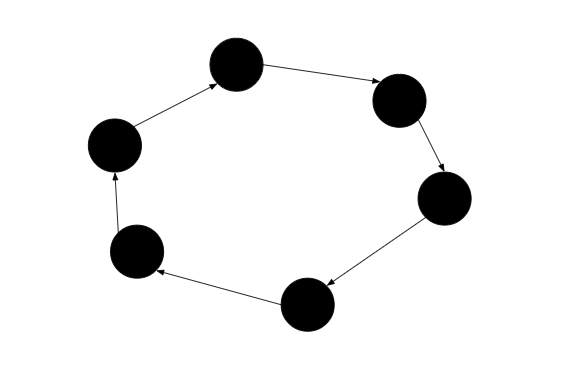
\includegraphics[scale=0.7]{../assets/dir_graph_1.png}
\end{center}

\subsubsection{Obstacle}
\begin{proposition}
    If $G$ is a directed graph with a cycle, then $G$ has no topological ordering.
\end{proposition}
So, in other words, if $G$ is a directed graph with at least one cycle \emph{anywhere}, then it has no topological ordering.

\begin{mdframed}[]
    \begin{proof}
        Suppose we have a cycle $v_1, \dots, v_n$. Assume for the sake of contradiction taht we have an ordering. Then, there are $n$ vertices so one of them has to come first; say that $v_i$ came first in the ordering. But, this is a cycle so there is an edge from $v_{i - 1}$ to $v_i$. However, because $v_i$ was first so it must come first in the order, in contradiction to the order property. 
    \end{proof}
\end{mdframed}

\subsection{Directed Acyclic Graph (DAG)}
Suppose we want to focus on directed graphs with no cycles. This brings us to the following definition.
\begin{definition}{}{}
    A \textbf{directed acylic graph} (DAG) is a directed graph which contains no cycles. 
\end{definition}

The previous result said that only DAGs can be topologically ordered. However, is the reverse true? That is, is it the case that every DAG has a topological ordering? \textbf{Yes}. 

\subsection{Existence of Orderings}
\begin{theorem}{}{}
    Let $G$ be a (finite) DAG. Then, $G$ has a topological ordering.
\end{theorem}

\begin{mdframed}[]
    \begin{proof}
        We consider the last vertex in the ordering; in other words, whatever vertex comes last in this ordering. This vertex must be a sink, or a vertex with no outgoing edges. So, once we find the sink, we can put the graph at the end of the topological graph, and then order the remaining vertices. Now, using the lemma below, we want to show that every DAG has a topological ordering. We will use induction on $|G|$. Omitting the base case, we find a sink $v$. Then, create a graph $G' = G \setminus \{v\}$. We can inductively order $G'$, which is still a DAG. Then, add $v$ to the end of the ordering. 
    \end{proof}
\end{mdframed}

\subsubsection{Sinks}
\begin{lemma}{}{}
    Every finite DAG contains at least one sink. 
\end{lemma}

\begin{mdframed}[]
    \begin{proof}
        Start at a vertex $v = v_1$. Then, we can ``follow the trail,'' or in other words follow the edges $(v_1, v_2)$, $(v_2, v_3)$, \dots. Eventually, we will either find: 
        \begin{itemize}
            \item Some vertices repeat (which creates a cycle). This can't happen if this is a DAG, though. 
            \item Or, we get stuck (which means we found a sink).
        \end{itemize}
        So, we are done. 
    \end{proof}
\end{mdframed}

\subsection{Algorithm}
Suppose we want to design an algorithm that, given a DAG $G$, computes a topological ordering on G. We can use the proof to create a naive algorithm. 
\begin{itemize}
    \item Find a sink $v$. This is done by following a chain of vertices until we are stuck.
    \item Compute the ordering on $G - \{v\}$.
    \item Place $v$ at the end. 
\end{itemize}
This algorithm can be written like so: 
\begin{verbatim}
    TopologicalOrdering(G)
        If |G| = 0
            Return {}
        Let v in G 
        While there is an edge (v, w)
            v = w
        Return (Ordering(G - v), v)
\end{verbatim}
The runtime is $O(|V|^2)$. This is because we need $|V|$ time to find each sink and have $|V|$ sinks. This is suboptimal, however. Consider this optimal algorithm:
\begin{verbatim}
    TopologicalOrdering(G)
        Run DFS(G) w/ Pre/Post Numbers 
        Return Vertices in Reverse Postorder
\end{verbatim}
This runs in $O(|V| + |E|)$.

\subsubsection{Example: DAG}
Consider the following DAG which we will call $G$:
\begin{center}
    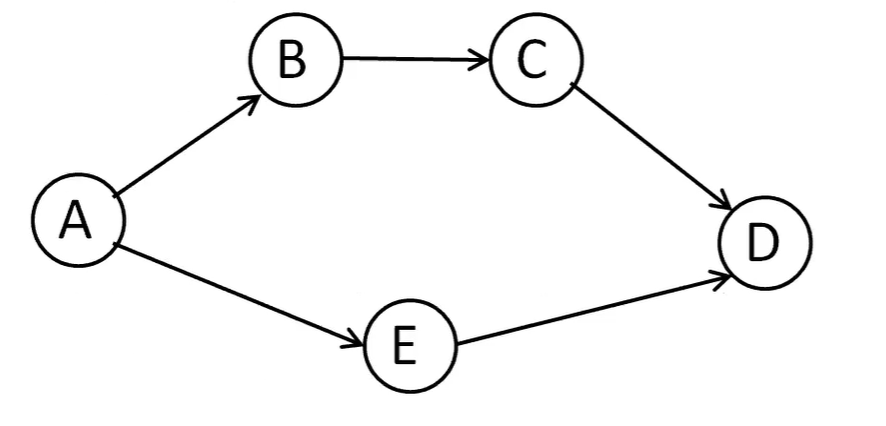
\includegraphics[scale=0.4]{../assets/dag_ex.png}
\end{center}
Suppose we start at $A$.
\begin{itemize}
    \item \underline{Using Algorithm 1:}
    \begin{itemize}
        \item First, we enumerate through the graph $G$ until we find a sink. In this case:
        \[A \mapsto B \mapsto C \mapsto D\]
        \item We \emph{remove} $D$ from the graph and add it to the ordering.
        \begin{verbatim}
            D
        \end{verbatim}
        \item Now, we enumerate through the graph $G - \{D\}$. In this case:
        \[A \mapsto B \mapsto C\]
        \item We \emph{remove} $C$ from the graph and add it to the ordering. 
        \begin{verbatim}
            C -> D
        \end{verbatim}
        \item Now, we enumerate through the graph $G - \{C, D\}$. In this case: 
        \[A \mapsto B\]
        \item We \emph{remove} $B$ from the graph and add it to the ordering. 
        \begin{verbatim}
            B -> C -> D
        \end{verbatim}
        \item Now, we enumerate through the graph $G - \{B, C, D\}$. In this case: 
        \[A \mapsto E\]
        \item We \emph{remove} $E$ from the graph and add it to the ordering. 
        \begin{verbatim}
            E -> B -> C -> D
        \end{verbatim}
        \item As we only have $A$ left, we can add it to the ordering. 
        \begin{verbatim}
            A -> E -> B -> C -> D
        \end{verbatim}
        So, we are done. 
    \end{itemize}

    \item \underline{Using Algorithm 2:}
    \begin{itemize}
        \item First, we enumerate through the graph $G$ until we find a sink. In this case: 
        \[A \mapsto B \mapsto C \mapsto D\]
        \item We remove $D$ from the graph and add it to the ordering. 
        \begin{verbatim}
            D
        \end{verbatim}
        \item Now, we remember that we already made it to $C$ and that $C$ is a sink in $G - \{D\}$. So, we remove $C$ and add it to the ordering: 
        \begin{verbatim}
            C -> D
        \end{verbatim}
        \item We remember that we already made it to $B$ and that $B$ is a sink in $G - \{C, D\}$. So, we remove $B$ and add it to the ordering: 
        \begin{verbatim}
            B -> C -> D
        \end{verbatim}
        \item Now that we're back at $A$, we note that $A$ has another edge. So, we go to that edge until we find a sink. In this case: 
        \[A \mapsto E\]
        \item We remove $E$ from the graph and add it to the ordering. 
        \begin{verbatim}
            E -> B -> C -> D
        \end{verbatim}
        \item Now, $A$ is the only vertex left in $G - \{B, C, D, E\}$. So, we add it to the ordering:
        \begin{verbatim}
            A -> E -> B -> C -> D
        \end{verbatim}
    \end{itemize}
    Here, we notice that algorithm 2 resembles depth-first seearch!
\end{itemize}

Another way to find a topological ordering for this graph is to consider the in-degrees of each vertex; i.e. the number of edges connecting \textbf{to} it. If we label each of $G$'s vertices with its in-degrees, we will have: 
\begin{center}
    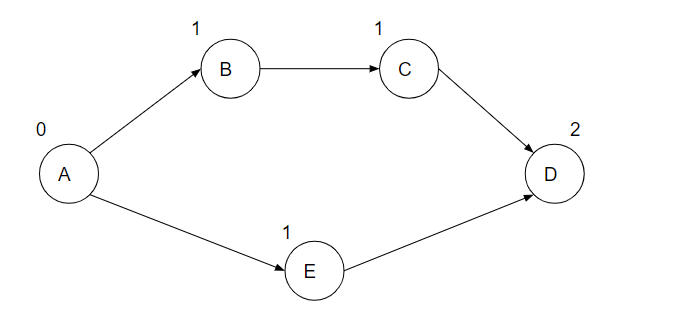
\includegraphics[scale=0.7]{../assets/dag_ex_deg_1.png}
\end{center}
So, this makeshift algorithm is essentially:
\begin{verbatim}
    TopologicalOrdering(G)
        ordering = []
        while G is not empty
            v = vertex in G with lowest in-degree (i.e. in-degree 0)
            ordering.append(v)
            Remove v from G
            Update in-degrees of existing vertices
        return ordering  
\end{verbatim}
\begin{itemize}
    \item First, note that $A$ has the lowest in-degree. So, remove $A$ from the graph and add it to the ordering. The ordering now looks like: 
    \begin{verbatim}
        [A]
    \end{verbatim}
    \item The graph now looks like: 
    \begin{center}
        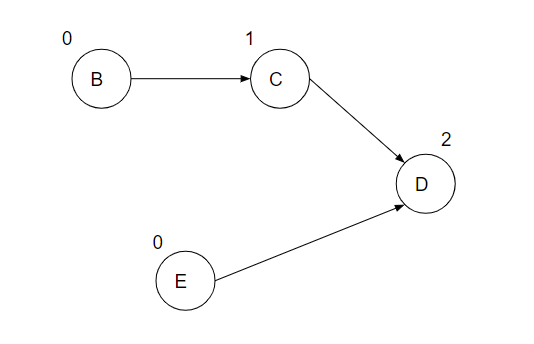
\includegraphics[scale=0.4]{../assets/dag_ex_deg_2.png}
    \end{center}
    Here, $B$ and $E$ both have the lowest in-degree. So, we can remove one or the other. For the sake of consistency, remove $E$ from the graph and add it to the ordering. The ordering now looks like: 
    \begin{verbatim}
        [A, E]
    \end{verbatim}
    \item The graph now looks like:
    \begin{center}
        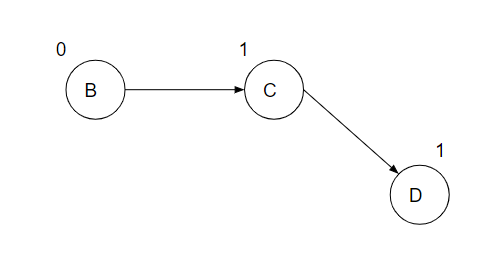
\includegraphics[scale=0.4]{../assets/dag_ex_deg_3.png}
    \end{center}
    Here, note that $B$ is the only node with the lowest in-degree. So, we remove it and add it to the ordering. The ordering now looks like: 
    \begin{verbatim}
        [A, E, B]
    \end{verbatim}
    \item The graph now looks like:
    \begin{center}
        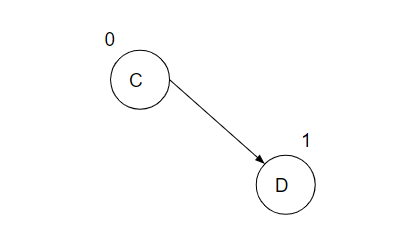
\includegraphics[scale=0.4]{../assets/dag_ex_deg_4.png}
    \end{center}
    Here, $C$ has the lowest in-degree so we remove it and add it to the ordering. The ordering now looks like: 
    \begin{verbatim}
        [A, E, B, C]
    \end{verbatim}
    \item By now, it's trivial to see that $D$ has in-degree 0, so we add it.
    \begin{verbatim}
        [A, E, B, C, D]
    \end{verbatim}
    And we are done. 
\end{itemize}

\subsection{Topological Sort}
This is a particularly useful algorithm. 
\begin{itemize}
    \item Many graph algorithms are relatively easy to find the answer for $v$ if you've already found the answer for everything downstream of $v$. 
    \begin{itemize}
        \item We can topologically sort $G$. 
        \item Then, solve for $v$ in reverse topological order.
    \end{itemize}
\end{itemize}

\subsection{Connectivity in Digraphs}
In undirected graphs, we had a very clean description of reachability: $v$ was reachable from $w$ if and only if they were in the same connected component. Well, this no longer works for digraphs. 

\end{document}